\section{Experiments}
We conduct comprehensive experiments to evaluate the effectiveness of \method~on both simulation benchmarks and real-world robotic manipulation tasks.
Our experiments are designed to answer the following research questions:

\noindent
\textbf{(RQ1)} How does \method~compare with recent state-of-the-art VLA methods on CALVIN and LIBERO benchmarks (see \Cref{sec:sota,sec:benchmark})?



\noindent
\textbf{(RQ2)} What empirical insights can guide key design choices for \method, including schedule hyperparameters $c$ and $\alpha$, two-stage decoding allocation, and velocity-field construction (see \Cref{sec:ablation})?

\noindent
\textbf{(RQ3)} What additional insights can we gain from in-depth analysis of decoding behavior, execution quality, and efficiency trade-offs (see \Cref{sec:analysis})?

\noindent
\textbf{(RQ4)} Can \method~generalize effectively to real-world manipulation tasks (see \Cref{sec:real})?


\subsection{Setup}
% \textbf{Implementation Details.}
% 我们采用与univla相同的backbone Emu3~

% For action modeling, we follow FAST and apply the Discrete Cosine Transform (DCT) to map continuous action trajectories into discrete action tokens.

We initialize our model from checkpoints pretrained on robotic video data~\citep{univla} and keep the remaining settings consistent with UniVLA.
Unless otherwise specified, we use a learning rate of $1\times10^{-4}$ and a batch size of 8.
All training and inference are conducted on 8 NVIDIA H100 GPUs.
For simulation benchmarks (CALVIN and LIBERO), we train for 20k--32k steps depending on the setting, while each real-world task is trained for 5k steps.
Unless otherwise noted, we follow~\citep{luo2025next} and use $c=3$ and $\alpha=1$ as the default setting. 
% We then conduct ablation studies on $c$ and $\alpha$ to quantify their effects on iterative refinement.



\subsection{Benchmarks}
\label{sec:benchmark}
\textbf{CALVIN.}
CALVIN~\citep{mees2022calvin} is a simulation benchmark for long-horizon, language-conditioned robotic manipulation, covering four environments (A, B, C, and D), 34 manipulation skills, and 1,000 language annotations. In this work, we follow the standard \textbf{ABCD$\rightarrow$D} setup. Concretely, each evaluation rollout contains a chain of five consecutive language-conditioned sub-tasks, and success on later sub-tasks depends on the correctness of earlier actions. This makes CALVIN particularly suitable for measuring error accumulation and temporal consistency in multi-step control. We evaluate 1,000 rollouts per model and report the average number of consecutively completed sub-tasks (Avg. Len., maximum 5), together with per-step completion rates.

\noindent
\textbf{LIBERO.}
LIBERO~\citep{liu2023libero} is a simulation benchmark designed to stress-test cross-task generalization along multiple dimensions. It is organized into four suites: Spatial, Object, Goal, and Long. Spatial focuses on spatial-relation understanding under varied layouts, Object emphasizes object-level generalization, Goal evaluates goal-conditioned manipulation under different target configurations, and Long tests long-horizon compositional reasoning over multi-stage behaviors. Compared with CALVIN, LIBERO places stronger emphasis on broad generalization across task families. We report per-suite success rates and the overall average. Each suite contains 10 tasks, with 50 evaluation rollouts per task.

\subsection{Comparison with SOTA}
\label{sec:sota}


We report the main results on CALVIN and LIBERO in \Cref{tab:calvin_results,tab:libero}. On CALVIN, both variants of \method~ outperform most strong VLA baselines, and \method+Embed achieves the best overall average length of 4.44. 
Compared with unified AR VLAs (e.g., UniVLA$^{*}$), \method+Embed improves 3-step and 5-step completion (0.892 vs. 0.862 and 0.780 vs. 0.690), indicating stronger long horizon consistency. It also outperforms continuous diffusion VLA models across all reported metrics, showing that discrete action refinement is competitive with optimization in continuous action spaces. Moreover, compared with AR baselines that enhance perception, such as ReconVLA, our method delivers gains of 0.19, showing that focused action iterative refinement is more effective. 
Although \method+Head is slightly weaker than \method+Embed, it still surpasses other baselines, further supporting the robustness of velocity guided action regeneration in long-horizon tasks.


% We also observe that \method+Head attains the best 4-task completion rate (0.864), suggesting that explicit velocity-head modeling brings additional robustness in mid-horizon planning.

On LIBERO, our method shows clear gains across all suites. \method+Embed reaches the best overall average success rate of 95.7\%, surpassing reasoning-guided discrete VLAs that rely on text or spatial chain of thought cues, for example, ThinkAct, MolmoAct, and CoT-VLA. It also improves over DreamVLA, which follows continuous diffusion with future visual prediction, by +3.1 points, and over FlowVLA, which uses autoregressive future optical flow cues, by +7.6 points. In particular, it achieves the highest scores on Object at 98.8\% and Long at 92.6\%, while maintaining strong performance on Spatial and Goal tasks. These results suggest that directly refining actions with previously generated coarse action signals is more effective than relying on auxiliary modality chain of thought guidance, leading to better long-horizon execution and cross-task generalization.

\begin{figure}[t]
    \centering
    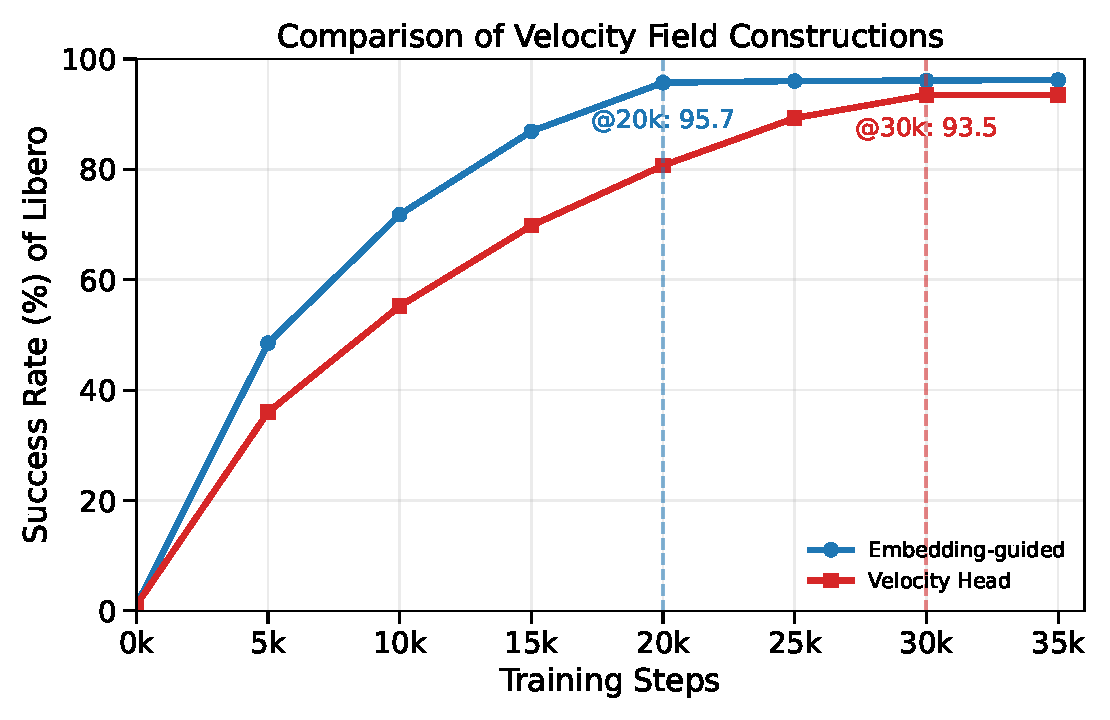
\includegraphics[width=0.8\linewidth]{figure/velocity_field_compare.pdf}
    \caption{Comparison of velocity field constructions across training steps. The Embedding-guided variant consistently outperforms the Velocity Head variant in both convergence speed and final performance, reaching a state-of-the-art success rate of 95.7\% on LIBERO with only 20k training steps.}
    \label{fig:velocity_field_compare}
\end{figure}
\subsection{Ablation Studies}
\label{sec:ablation}
We conduct ablation studies to isolate the effects of key design and training choices, including schedule hyperparameters $c$ and $\alpha$, two-stage decoding step allocation, and velocity-field construction. Detailed quantitative results are summarized in \Cref{tab:ablation_lambda_c_alpha,tab:ablation_two_stage,fig:velocity_field_compare}.


\begin{wraptable}{r}{0.48\textwidth}
    \vspace{-10mm}
    \centering
    \footnotesize
    \setlength{\tabcolsep}{4pt}
    \caption{Ablation study on $c$ and $\alpha$.}
    \label{tab:ablation_lambda_c_alpha}
    \begin{tabular}{c|c|c|c}
        \toprule
        $c$ & $\alpha$ & CALVIN $\uparrow$ & LIBERO (\%) $\uparrow$ \\
        \midrule
        1 & 1 & 4.38 & 95.0 \\
        3 & 1 & 4.44 & 95.7 \\
        5 & 1 & 4.40 & 95.2 \\
        3 & 0.5 & 4.40 & 95.6 \\
        \bottomrule
    \end{tabular}
    \vspace{-5mm}
\end{wraptable}

\paragraph{Effect of $c$ and $\alpha$.}
In Eq.~\ref{eq:beta_t}, $c$ controls the overall scale of $\beta_t$, while $\alpha$ controls the temporal curvature of the schedule, determining how quickly refinement concentrates as $t\!\to\!1$.
\Cref{tab:ablation_lambda_c_alpha} shows that \method~is robust to moderate changes of both parameters, with $c=3,\alpha=1$ giving the best  trade-off.
Under this setting, \method~achieves the  Avg. Len. of 4.44 on CALVIN and average success rate of 95.7\% on Libero. 
Increasing $c$ to 5 or decreasing $\alpha$ to 0.5 causes only minor fluctuations, indicating stable refinement dynamics across a reasonably wide hyperparameter region.

\begin{wraptable}{r}{0.5\textwidth}
    \vspace{-10mm}
    \centering
    \footnotesize
    \setlength{\tabcolsep}{5pt}
    \caption{Ablation on two-stage decoding step allocation with fixed total steps ($T_{\mathrm{fine}} + T_{\mathrm{val}} = 16$).}
    \label{tab:ablation_two_stage}
    \begin{tabular}{c | c | c |c}
        \toprule
        $T_{\mathrm{fine}}$ & $T_{\mathrm{val}}$ & CALVIN $\uparrow$ & LIBERO (\%) $\uparrow$ \\
        \midrule
        16 & 0  & 4.37 & 94.8 \\
        15 & 1  & 4.39 & 95.2 \\
        14 & 2  & \textbf{4.44} & \textbf{95.7} \\
        12 & 4  & 4.41 & 95.4 \\
        8  & 8  & 4.35 & 95.1 \\
        \bottomrule
    \end{tabular}
    \vspace{-3mm}
\end{wraptable}
\paragraph{Effect of Two-Stage Decoding.}
We further ablate how decoding steps are allocated between the iterative refinement stage ($T_{\mathrm{fine}}$) and the deterministic validation stage ($T_{\mathrm{val}}$). We keep the total number of steps fixed at 16 and report Avg. Len. of CALVIN ABCD$\rightarrow$D  and average success rate of LIBERO in \Cref{tab:ablation_two_stage}. As shown in the table, using only iterative refinement  ($T_{\mathrm{val}}=0$) yields weaker performance. Introducing a short validation stage improves both benchmarks, and $T_{\mathrm{fine}}=14, T_{\mathrm{val}}=2$ achieves the best overall trade-off. In contrast, allocating too many steps to the validation stage slightly hurts action quality, suggesting that excessive early greedy release reduces refinement flexibility. Therefore, we use $T_{\mathrm{fine}}=14$ and $T_{\mathrm{val}}=2$ in all experiments.



\paragraph{Comparison of Velocity Field Constructions.}
To further analyze the effect of velocity-field design, we compare the embedding-guided formulation with the head-based formulation across training steps. As shown in~\Cref{fig:velocity_field_compare}, the embedding-guided variant converges faster in the early stages of training and consistently reaches better final task performance. This trend indicates that embedding guidance provides more informative and smooth optimization signals, leading to both improved data efficiency and a stronger final policy.




\subsection{In-Depth Analysis}
\label{sec:analysis}

% \begin{wraptable}{r}{0.5\textwidth}
%     \vspace{-10mm}
%     \centering
%     \footnotesize
%     \setlength{\tabcolsep}{2pt}
%     \caption{Inference efficiency comparison across AR, DD and DFM on CALVIN ABCD$\rightarrow$D. DD and DFM use the same decoding steps (16).}
%     \label{tab:efficiency_main}
%     \begin{tabular}{lcc}
%         \toprule
%         Method & Avg. Len. $\uparrow$ & Speed $\uparrow$ \\
%         \midrule
%         AR & 4.18 & 50.2  \\
%         DD & 4.32 & 62.1  \\
%         DD + Adap. Cache & 4.27 & 118.3  \\
%         DFM & 4.42 & 60.2  \\
%         DFM + Adap. Cache & 4.40 & 121.0  \\
%         \bottomrule
%     \end{tabular}
%     \vspace{-6mm}
% \end{wraptable}
\paragraph{Effectiveness of Decoding Method.}

\begin{table*}[t]
    \centering
    \footnotesize
    \begin{minipage}[t]{0.47\textwidth}
        \centering
        \setlength{\tabcolsep}{2pt}
        \caption{Inference efficiency comparison across AR, DD, and DFM on CALVIN ABCD$\rightarrow$D. DD and DFM use the same decoding steps (16).}
        \label{tab:efficiency_main}
        \begin{tabular}{l|c|c}
            \toprule
            Method & Avg. Len. $\uparrow$ & Speed $\uparrow$ \\
            \midrule
            AR & 4.18 & 50.2  \\
            DD & 4.32 & 62.1  \\
            DD + Adap. Cache & 4.27 & 118.3  \\
            DFM & \textbf{4.42} & 60.2  \\
            DFM + Adap. Cache & 4.40 & \textbf{121.0}  \\
            \bottomrule
        \end{tabular}
    \end{minipage}\hfill
    \begin{minipage}[t]{0.47\textwidth}
        \centering
        \setlength{\tabcolsep}{2pt}
        \caption{Ablation on training data scale on CALVIN ABCD$\rightarrow$D . We compare three discrete VLA paradigms across data scales, with DD and DFM evaluated using the same number of decoding steps.}
        \label{tab:ablation_data_scale}
        \begin{tabular}{c|ccc}
            \toprule
            Data Fraction & AR & DD & DFM (Ours) \\
            \midrule
            10\%  & 1.71 & 2.84 & \textbf{3.21}   \\
            50\%  & 3.01 & 3.88 & \textbf{4.03}   \\
            100\% & 4.18 & 4.32 & \textbf{4.44}   \\
            \bottomrule
        \end{tabular}
    \end{minipage}
\end{table*}
We keep the architecture unchanged and compare AR, DD, and our method, while also validating the effectiveness of Adaptive Cache in inference.
Results in \Cref{tab:efficiency_main} show that \method~achieves the best action quality among the compared decoding strategies. With Adaptive Cache enabled, both DD and DFM obtain clear speedups, and \textit{DFM+Adaptive Cache} delivers the fastest decoding while maintaining strong performance. These results indicate that DFM provides a favorable quality--efficiency trade-off under matched decoding steps.

% \begin{wraptable}{r}{0.5\textwidth}
%     \vspace{-8mm}
%     \centering
%     \footnotesize
%     \setlength{\tabcolsep}{4pt}
%     \caption{Ablation on training data scale on CALVIN ABCD$\rightarrow$D (Avg. Len. $\uparrow$). We compare three discrete VLA paradigms across data scales, with DD and DFM evaluated using the same number of decoding steps.}
%     \label{tab:ablation_data_scale}
%     \begin{tabular}{c|ccc}
%         \toprule
%         Data Fraction & AR & DD & DFM (Ours) \\
%         \midrule
%         10\%  & 1.71 & 2.84 & 3.21   \\
%         50\%  & 3.01 & 3.88 & 4.03   \\
%         100\% & 4.18 & 4.32 & 4.44   \\
%         \bottomrule
%     \end{tabular}
%     \vspace{-7mm}
% \end{wraptable}
\paragraph{Effect of training data size.}
\Cref{tab:ablation_data_scale} shows that \method~consistently outperforms both autoregressive and discrete diffusion baselines across all data scales on CALVIN ABCD$\rightarrow$D.
At 10\% data, \method~ achieves an Avg. Len. of 3.21, outperforming AR at 1.71 and discrete diffusion at 2.84 by +1.50 and +0.37, respectively. It also remains the best at 50\% data with 4.03 and at 100\% data with 4.44, showing consistent gains as data scale increases.
These results indicate that DFM-VLA is particularly beneficial in low-data regimes while maintaining consistent advantages as training data scales up.



\subsection{Real World Experiment}
\begin{figure}[t]
    \centering
    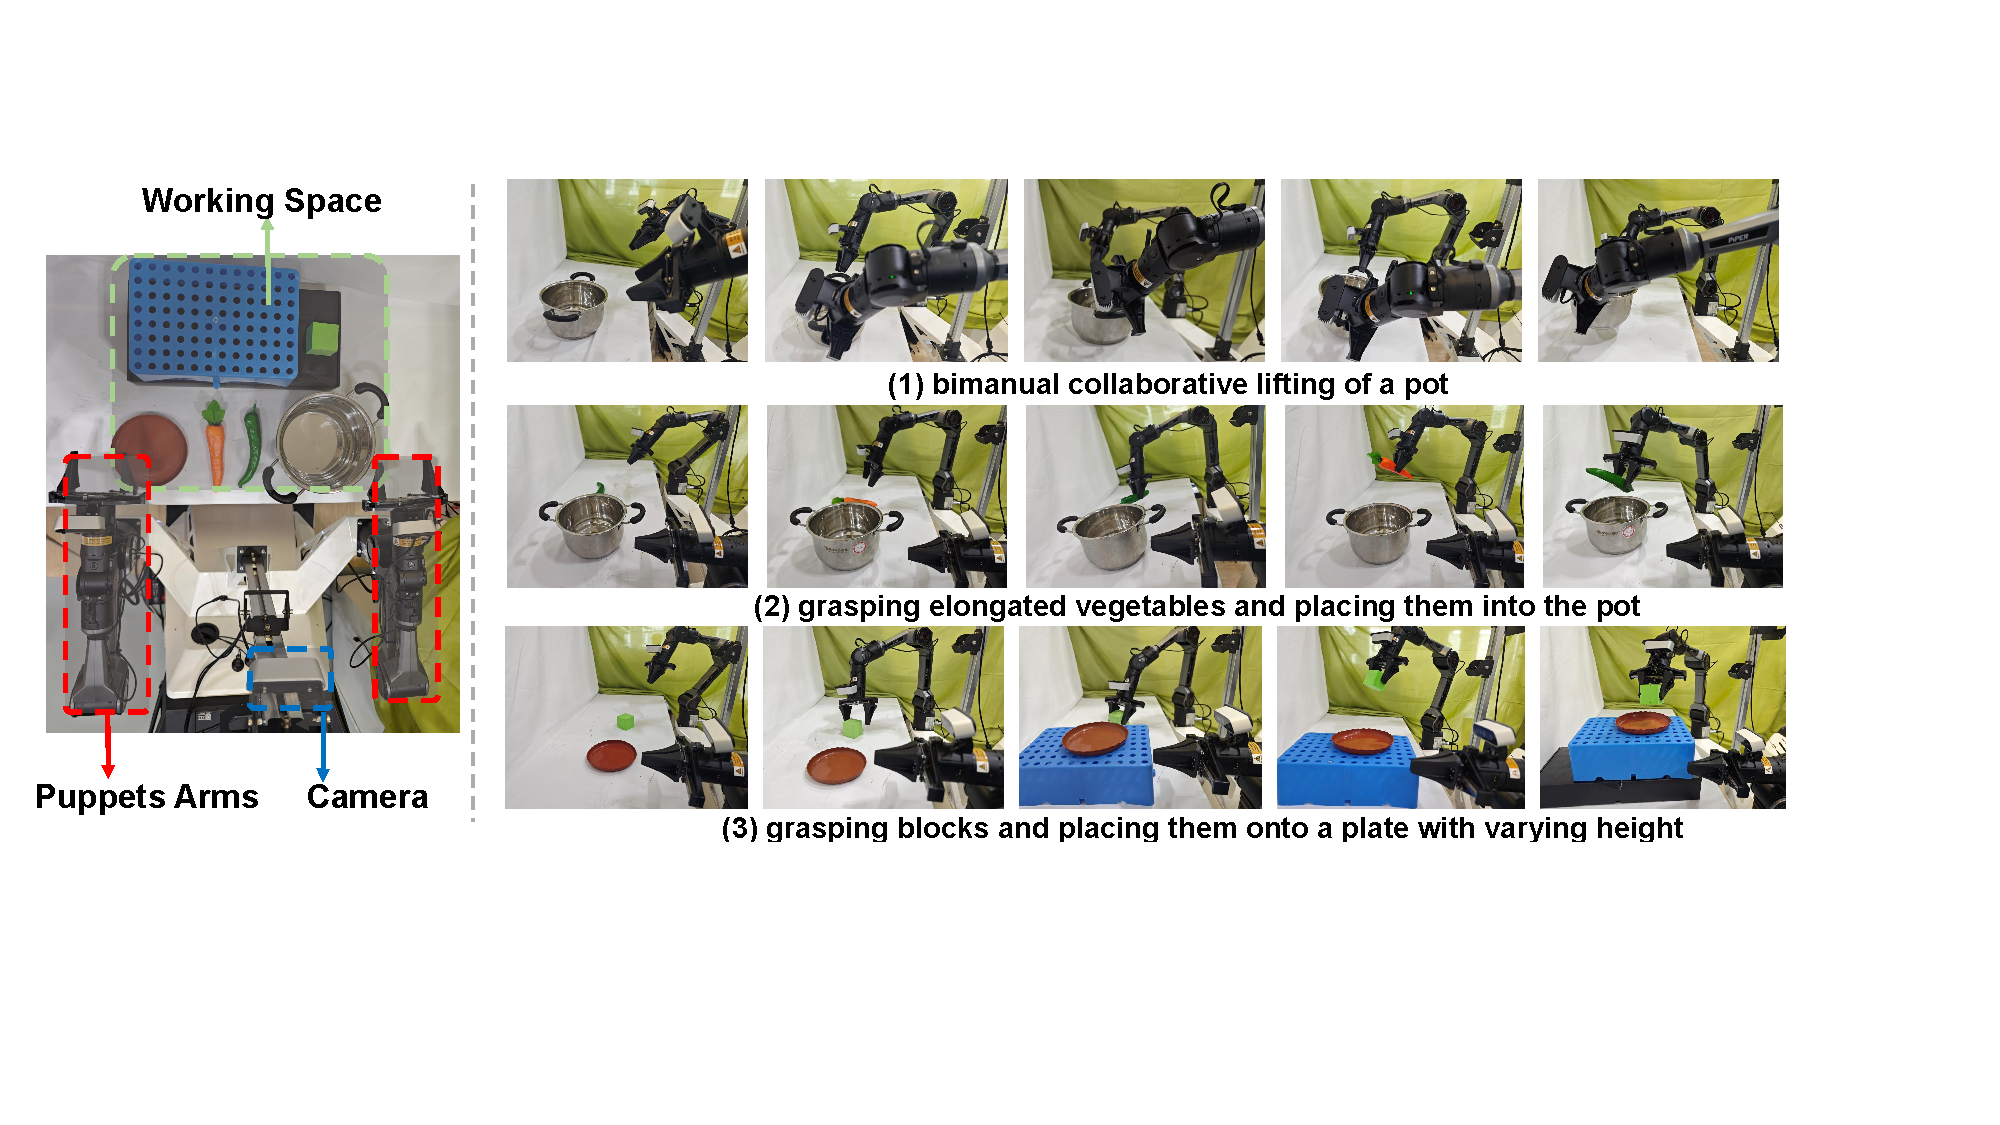
\includegraphics[width=0.99\linewidth]{figure/real_set.pdf}
    \caption{\textbf{Left:} The real-world robotic system for experiments.  \textbf{Right:} The representative task demonstrations.}

    \label{fig:real}
\end{figure}
%Setup.我们的真机实验在bimanual AgileX上进行，它具有两条机械臂，每条臂具有六个自由的的关节和一个夹爪。该机器具有三个摄像头：一个在机器中间高处视角，其余两个各自在机械臂的手腕上。
%Task Setting.我们一共设置了三个任务，如图所示，第一个任务是双臂协作举起锅；第二个是夹取条状蔬菜到锅中，蔬菜的位置和位姿会有所改变；第三个是夹取方块到盘子里，其中盘子的高度会进行改变。对于每个任务，我们均收集xx条数据进行训练，对于评估，我们对每个任务进行了四十次评估，记录他们的成功率以及完成速度。
\textbf{Setup.}
As shown in \Cref{fig:real}, 
we conduct real-world experiments on a bimanual AgileX platform equipped with two robotic arms, each with six degrees of freedom and a parallel gripper.
The system is instrumented with three RGB cameras: one fixed camera mounted at an elevated central viewpoint and two wrist-mounted cameras, one on each arm.

\noindent
\textbf{Task Setting.}
We design three representative manipulation tasks:
(1) bimanual collaborative lifting of a pot (\textit{Pot Lift});
(2) grasping elongated vegetables and placing them into the pot, where the object position and pose are varied (\textit{Place Veg. to Pot});
and (3) grasping a block and placing it onto a plate with varying height (\textit{Place Block to Plate}).
For each task, we collect 100 trajectories for training.
During evaluation, we run 40 trials per task and report both task success rate and completion speed.
\label{sec:real}

\noindent
\textbf{Results.}
We compare \method against representative methods from three action-generation paradigms for real-world manipulation: the autoregressive baseline $\pi_0$-FAST, the discrete diffusion baseline Dream-VLA, and the continuous diffusion baseline RDT~\citep{liu2024rdt}.
Table~\ref{tab:real_world_results} shows that \method~achieves the highest success rate on each task. Specifically, our \method~reaches a success rate of 77.5\% on \textit{Pot Lift}, which requires precise bimanual coordination; 70.0\% on \textit{Place Veg. to Pot}, which tests generalization to object positions and poses; and 65.0\% on \textit{Place Block to Plate}, which emphasizes spatial precision under varying plate heights. Overall, the average success rate of~\method~is 70.8\%, which surpasses RDT at 60.0\% by 10.8 percentage points and Dream-VLA at 54.2\% by 16.6 percentage points.

This result demonstrates that traditional discrete baselines (i.e., $\pi_0$-FAST and Dream-VLA) are weaker than the continuous diffusion baseline RDT because wrongly decoded action tokens cannot be refined, leading to error accumulation. 
In contrast, our method uses refined action guided by velocities over discrete action tokens to correct errors in time.
Meanwhile, its unified discrete input-output space better preserves semantic understanding from autoregressive VLM backbones~\citep{liang2025discrete,wen2025dvla}, yielding the best overall performance.
These results further show that action refinement with discrete flow matching remains highly competitive and robust in real-world settings.

\begin{table}[t]
    \centering
    \footnotesize
    \setlength{\tabcolsep}{3pt}
    \caption{Real-world success rate comparison (\%) on three tasks.}
    \label{tab:real_world_results}
    \begin{tabular}{lccc|c}
        \toprule
        Method & Pot Lift & Place Veg. to Pot & Place Block to Plate & Average \\
        \midrule
        $\pi_0$-FAST~\citep{pertsch2025fast} & 50.0 & 42.5 & 35.0 & 42.5 \\
        Dream-VLA~\citep{yedreamVLA} & 57.5 & 62.5  & 42.5  & 54.2 \\
        RDT~\citep{liu2024rdt} & 65.0 & 62.5  & 52.5  & 60.0 \\
         \rowcolor[gray]{0.9}
        \textbf{\method+Head} & 70.0 & 67.5  & 60.0 & 65.8 \\
        \rowcolor[gray]{0.9}
        \textbf{\method+Embed} & \textbf{77.5}  & \textbf{70.0} & \textbf{65.0} & \textbf{70.8} \\
        \bottomrule
    \end{tabular}
\end{table}




